\documentclass{article}
\usepackage{graphicx} % Required for inserting images
\usepackage[T2A]{fontenc}
\usepackage{titlesec}
%\usepackage{verbatim}
\usepackage[left=25mm, right=15mm, top=20mm, bottom=20mm, footskip=10mm]{geometry}
\usepackage{amsmath}
\usepackage{epigraph}
\usepackage{tikz}
\usepackage{latexsym}
%\usepackage{listings}
\frenchspacing 
\newcommand{\path}{\rightsquigarrow}
\titleformat{\section}[hang]{\normalsize\bfseries}{\thesection~}{0pt}{}
\titlespacing{\section}{\parindent}{\baselineskip}{\baselineskip}

\titleformat{\subsection}[hang]{\normalsize}{\thesubsection~}{0pt}{}
\titlespacing{\subsection}{\parindent}{0pt}{0pt}
\parindent=1.25cm 

\title{Тема 6. Динамическое программирование }
\date{}

\begin{document}

\maketitle

\epigraph{Автор конспекта: Родион Лыков}

Давайте рассмотрим следующую задачу: вам дан ориентированный граф без циклов. У каждого ребра есть стоимость прохода по этому ребру. Вам нужно найти путь из вершин $1$ в $n$ с максимальной стоимостью. Например, в следущем графе ответ  

\begin{center}
        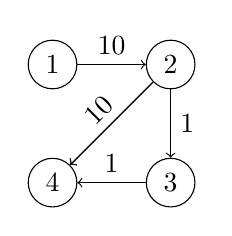
\begin{tikzpicture}[main/.style = {draw, circle},node distance={15mm}] 
        \node[main] (1) []{$1$}; 
        \node[main] (2) [right of=1] {$2$}; 
        \node[main] (3) [below of=2] {$3$}; 
        \node[main] (4) [left of=3] {$4$};
        \draw[->] (1) -> (2) node [midway, above] {$10$};
        \draw[->] (2) -> (3) node [midway, right] {$1$};
        \draw[->] (2) -> (4);
        \draw[->] (2) -- node[midway, above right, sloped, pos=0.7] {$10$} (4);
        \draw[->] (3) -> (4) node [midway, above] {$1$};
        \end{tikzpicture} 
    \end{center}

Здесь самый максимальный путь будет $1 \rightarrow 2, 2 \rightarrow 4$ и имеет стоимость $20$. Как видите, не всегда самый длинный путь будет иметь максимальную стоимость.
Но если вы подумали, что мы можем идти по самому дорогому ребру каждый раз, то это тоже неправильно, например:

\begin{center}
        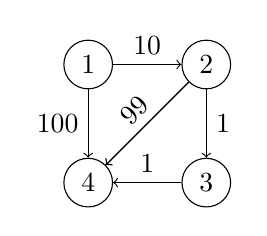
\begin{tikzpicture}[main/.style = {draw, circle},node distance={15mm}] 
        \node[main] (1) []{$1$}; 
        \node[main] (2) [right of=1] {$2$}; 
        \node[main] (3) [below of=2] {$3$}; 
        \node[main] (4) [left of=3] {$4$};
        \draw[->] (1) -> (2) node [midway, above] {$10$};
        \draw[->] (2) -> (3) node [midway, right] {$1$};
        \draw[->] (2) -> (4);
        \draw[->] (2) -- node[midway, above right, sloped, pos=0.7] {$99$} (4);
        \draw[->] (3) -> (4) node [midway, above] {$1$};
        \draw[->] (1) -> (4) node [midway, left] {$100$};
        \end{tikzpicture} 
    \end{center}
Если мы пойдем по самому дорогому ребру, то мы найдем число $100$ как самый большой путь, но ответ $109$,можно также пойти из $1$ в $2$, потом из $2$ в $4$. 

Итак, чтобы решить такую задачу мы можем ввести такой трюк: пусть $d[x]$ это максимальный путь, по которому мы можем попасть в $x$. Тогда, если мы научимся это считать, то $d[n]$ это ответ на задачу (нас же просили найти максимальный путь в $n$, что такое $d[n]$? Это максимальный путь, по которому мы можем попасть в $n$). Давайте посмотрим, как будет выглядеть это на графе:

\begin{center}
        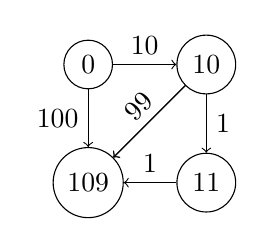
\begin{tikzpicture}[main/.style = {draw, circle},node distance={15mm}] 
        \node[main] (1) []{$0$}; 
        \node[main] (2) [right of=1] {$10$}; 
        \node[main] (3) [below of=2] {$11$}; 
        \node[main] (4) [left of=3] {$109$};
        \draw[->] (1) -> (2) node [midway, above] {$10$};
        \draw[->] (2) -> (3) node [midway, right] {$1$};
        \draw[->] (2) -> (4);
        \draw[->] (2) -- node[midway, above right, sloped, pos=0.7] {$99$} (4);
        \draw[->] (3) -> (4) node [midway, above] {$1$};
        \draw[->] (1) -> (4) node [midway, left] {$100$};
        \end{tikzpicture} 
    \end{center}
В вершинах записаны сами значения массива $d$. Так, $d[1] = 0$, ведь чтобы добраться из $1$ в $1$ по самому большому пути это $0$. Допустим, ответ для вершины $4$ еще мы не посчитали, массив $d$ выглядит так:

\begin{center}
        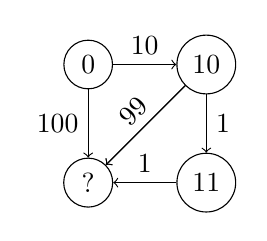
\begin{tikzpicture}[main/.style = {draw, circle},node distance={15mm}] 
        \node[main] (1) []{$0$}; 
        \node[main] (2) [right of=1] {$10$}; 
        \node[main] (3) [below of=2] {$11$}; 
        \node[main] (4) [left of=3] {?};
        \draw[->] (1) -> (2) node [midway, above] {$10$};
        \draw[->] (2) -> (3) node [midway, right] {$1$};
        \draw[->] (2) -> (4);
        \draw[->] (2) -- node[midway, above right, sloped, pos=0.7] {$99$} (4);
        \draw[->] (3) -> (4) node [midway, above] {$1$};
        \draw[->] (1) -> (4) node [midway, left] {$100$};
        \end{tikzpicture} 
    \end{center}
Теперь смотрите: попасть в $4$ можно по ребрам $(1,4,100), (2, 4, 99), (3, 4, 1)$. 
Давайте просто выберем самый оптимальный путь: $d[2] = 10, d[2] + 99 = 109$, именно так мы и посчитали путь до вершины $4$, если посчитаны все пути по остальным вершинам. То есть мы будем заполнять массив $d$ по очереди для всех вершин:

\begin{center}
        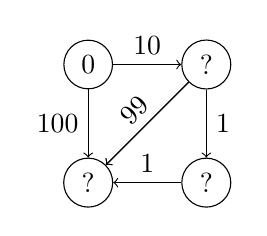
\begin{tikzpicture}[main/.style = {draw, circle},node distance={15mm}] 
        \node[main] (1) []{$0$}; 
        \node[main] (2) [right of=1] {?}; 
        \node[main] (3) [below of=2] {?}; 
        \node[main] (4) [left of=3] {?};
        \draw[->] (1) -> (2) node [midway, above] {$10$};
        \draw[->] (2) -> (3) node [midway, right] {$1$};
        \draw[->] (2) -> (4);
        \draw[->] (2) -- node[midway, above right, sloped, pos=0.7] {$99$} (4);
        \draw[->] (3) -> (4) node [midway, above] {$1$};
        \draw[->] (1) -> (4) node [midway, left] {$100$};
        \end{tikzpicture} 
    \end{center}
    \begin{center}
        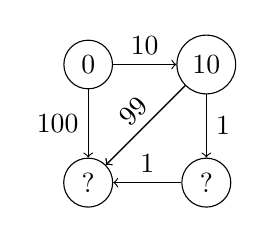
\begin{tikzpicture}[main/.style = {draw, circle},node distance={15mm}] 
        \node[main] (1) []{$0$}; 
        \node[main] (2) [right of=1] {$10$}; 
        \node[main] (3) [below of=2] {?}; 
        \node[main] (4) [left of=3] {?};
        \draw[->] (1) -> (2) node [midway, above] {$10$};
        \draw[->] (2) -> (3) node [midway, right] {$1$};
        \draw[->] (2) -> (4);
        \draw[->] (2) -- node[midway, above right, sloped, pos=0.7] {$99$} (4);
        \draw[->] (3) -> (4) node [midway, above] {$1$};
        \draw[->] (1) -> (4) node [midway, left] {$100$};
        \end{tikzpicture} 
    \end{center}
    \begin{center}
        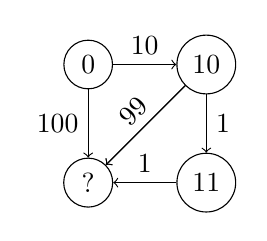
\begin{tikzpicture}[main/.style = {draw, circle},node distance={15mm}] 
        \node[main] (1) []{$0$}; 
        \node[main] (2) [right of=1] {$10$}; 
        \node[main] (3) [below of=2] {$11$}; 
        \node[main] (4) [left of=3] {?};
        \draw[->] (1) -> (2) node [midway, above] {$10$};
        \draw[->] (2) -> (3) node [midway, right] {$1$};
        \draw[->] (2) -> (4);
        \draw[->] (2) -- node[midway, above right, sloped, pos=0.7] {$99$} (4);
        \draw[->] (3) -> (4) node [midway, above] {$1$};
        \draw[->] (1) -> (4) node [midway, left] {$100$};
        \end{tikzpicture} 
    \end{center}
    \begin{center}
        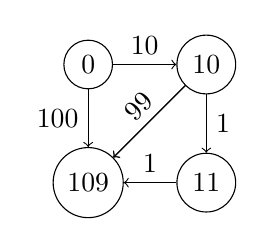
\begin{tikzpicture}[main/.style = {draw, circle},node distance={15mm}] 
        \node[main] (1) []{$0$}; 
        \node[main] (2) [right of=1] {$10$}; 
        \node[main] (3) [below of=2] {$11$}; 
        \node[main] (4) [left of=3] {$109$};
        \draw[->] (1) -> (2) node [midway, above] {$10$};
        \draw[->] (2) -> (3) node [midway, right] {$1$};
        \draw[->] (2) -> (4);
        \draw[->] (2) -- node[midway, above right, sloped, pos=0.7] {$99$} (4);
        \draw[->] (3) -> (4) node [midway, above] {$1$};
        \draw[->] (1) -> (4) node [midway, left] {$100$};
        \end{tikzpicture} 
    \end{center}

Давайте посмотрим пример на более сложном графе:

\begin{center}
        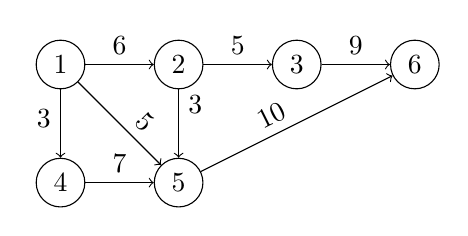
\begin{tikzpicture}[main/.style = {draw, circle},node distance={15mm}] 
        \node[main] (1) []{$1$}; 
        \node[main] (2) [right of=1] {$2$}; 
        \node[main] (3) [right of=2] {$3$}; 
        \node[main] (4) [below of=1] {$4$};
        \node[main] (5) [right of=4] {$5$};
        \node[main] (6) [right of=3] {$6$};
        \draw[->] (1) -- node[midway, above, sloped, pos=0.5] {$6$} (2);
        \draw[->] (2) -- node[midway, above, sloped, pos=0.5] {$5$} (3);
        \draw[->] (3) -- node[midway, above, sloped, pos=0.5] {$9$} (6);
        \draw[->] (1) -- node[midway, above left, pos=0.7] {$3$} (4);
        \draw[->] (1) -- node[midway, above right, sloped, pos=0.5] {$5$} (5);
        \draw[->] (4) -- node[midway, above, sloped, pos=0.5] {$7$} (5);
        \draw[->] (2) -- node[midway, above right, pos=0.5] {$3$} (5);
        \draw[->] (5) -- node[midway, above right, sloped, pos=0.3] {$10$} (6);
        \end{tikzpicture} 
    \end{center}
Давайте заполнять массив $d$ по очереди. А по какой очереди? По очереди топологической сортировки, конечно! Ведь когда мы идем из вершины, мы должны посмотреть все возможные пути для нее, ведь если мы не посмотрим все пути, мы просто не можем знать, что текущий найденный путь оптимальный!
\begin{center}
        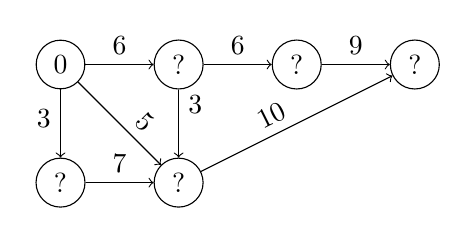
\begin{tikzpicture}[main/.style = {draw, circle},node distance={15mm}] 
        \node[main] (1) []{$0$}; 
        \node[main] (2) [right of=1] {?}; 
        \node[main] (3) [right of=2] {?}; 
        \node[main] (4) [below of=1] {?};
        \node[main] (5) [right of=4] {?};
        \node[main] (6) [right of=3] {?};
        \draw[->] (1) -- node[midway, above, sloped, pos=0.5] {$6$} (2);
        \draw[->] (2) -- node[midway, above, sloped, pos=0.5] {$6$} (3);
        \draw[->] (3) -- node[midway, above, sloped, pos=0.5] {$9$} (6);
        \draw[->] (1) -- node[midway, above left, pos=0.7] {$3$} (4);
        \draw[->] (1) -- node[midway, above right, sloped, pos=0.5] {$5$} (5);
        \draw[->] (4) -- node[midway, above, sloped, pos=0.5] {$7$} (5);
        \draw[->] (2) -- node[midway, above right, pos=0.5] {$3$} (5);
        \draw[->] (5) -- node[midway, above right, sloped, pos=0.3] {$10$} (6);
        \end{tikzpicture} 
    \end{center}
    \begin{center}
        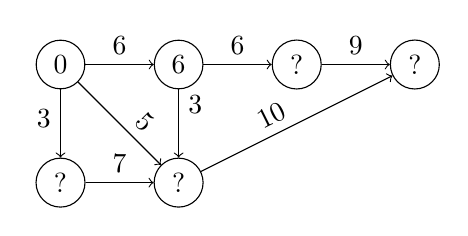
\begin{tikzpicture}[main/.style = {draw, circle},node distance={15mm}] 
        \node[main] (1) []{$0$}; 
        \node[main] (2) [right of=1] {$6$}; 
        \node[main] (3) [right of=2] {?}; 
        \node[main] (4) [below of=1] {?};
        \node[main] (5) [right of=4] {?};
        \node[main] (6) [right of=3] {?};
        \draw[->] (1) -- node[midway, above, sloped, pos=0.5] {$6$} (2);
        \draw[->] (2) -- node[midway, above, sloped, pos=0.5] {$6$} (3);
        \draw[->] (3) -- node[midway, above, sloped, pos=0.5] {$9$} (6);
        \draw[->] (1) -- node[midway, above left, pos=0.7] {$3$} (4);
        \draw[->] (1) -- node[midway, above right, sloped, pos=0.5] {$5$} (5);
        \draw[->] (4) -- node[midway, above, sloped, pos=0.5] {$7$} (5);
        \draw[->] (2) -- node[midway, above right, pos=0.5] {$3$} (5);
        \draw[->] (5) -- node[midway, above right, sloped, pos=0.3] {$10$} (6);
        \end{tikzpicture} 
    \end{center}
    \begin{center}
        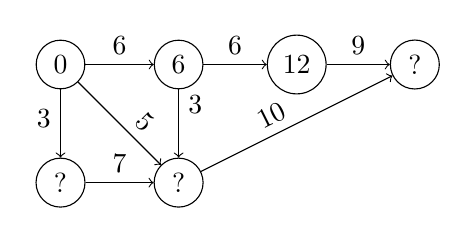
\begin{tikzpicture}[main/.style = {draw, circle},node distance={15mm}] 
        \node[main] (1) []{$0$}; 
        \node[main] (2) [right of=1] {$6$}; 
        \node[main] (3) [right of=2] {$12$}; 
        \node[main] (4) [below of=1] {?};
        \node[main] (5) [right of=4] {?};
        \node[main] (6) [right of=3] {?};
        \draw[->] (1) -- node[midway, above, sloped, pos=0.5] {$6$} (2);
        \draw[->] (2) -- node[midway, above, sloped, pos=0.5] {$6$} (3);
        \draw[->] (3) -- node[midway, above, sloped, pos=0.5] {$9$} (6);
        \draw[->] (1) -- node[midway, above left, pos=0.7] {$3$} (4);
        \draw[->] (1) -- node[midway, above right, sloped, pos=0.5] {$5$} (5);
        \draw[->] (4) -- node[midway, above, sloped, pos=0.5] {$7$} (5);
        \draw[->] (2) -- node[midway, above right, pos=0.5] {$3$} (5);
        \draw[->] (5) -- node[midway, above right, sloped, pos=0.3] {$10$} (6);
        \end{tikzpicture} 
    \end{center}
    \begin{center}
        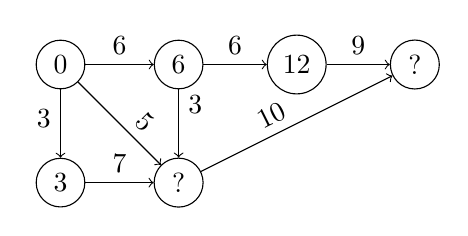
\begin{tikzpicture}[main/.style = {draw, circle},node distance={15mm}] 
        \node[main] (1) []{$0$}; 
        \node[main] (2) [right of=1] {$6$}; 
        \node[main] (3) [right of=2] {$12$}; 
        \node[main] (4) [below of=1] {$3$};
        \node[main] (5) [right of=4] {?};
        \node[main] (6) [right of=3] {?};
        \draw[->] (1) -- node[midway, above, sloped, pos=0.5] {$6$} (2);
        \draw[->] (2) -- node[midway, above, sloped, pos=0.5] {$6$} (3);
        \draw[->] (3) -- node[midway, above, sloped, pos=0.5] {$9$} (6);
        \draw[->] (1) -- node[midway, above left, pos=0.7] {$3$} (4);
        \draw[->] (1) -- node[midway, above right, sloped, pos=0.5] {$5$} (5);
        \draw[->] (4) -- node[midway, above, sloped, pos=0.5] {$7$} (5);
        \draw[->] (2) -- node[midway, above right, pos=0.5] {$3$} (5);
        \draw[->] (5) -- node[midway, above right, sloped, pos=0.3] {$10$} (6);
        \end{tikzpicture} 
    \end{center}
    \begin{center}
        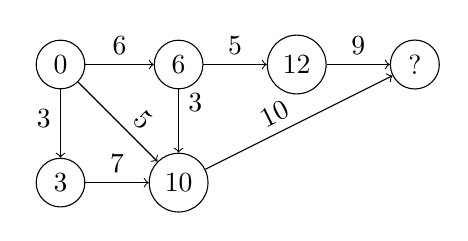
\begin{tikzpicture}[main/.style = {draw, circle},node distance={15mm}] 
        \node[main] (1) []{$0$}; 
        \node[main] (2) [right of=1] {$6$}; 
        \node[main] (3) [right of=2] {$12$}; 
        \node[main] (4) [below of=1] {$3$};
        \node[main] (5) [right of=4] {$10$};
        \node[main] (6) [right of=3] {?};
        \draw[->] (1) -- node[midway, above, sloped, pos=0.5] {$6$} (2);
        \draw[->] (2) -- node[midway, above, sloped, pos=0.5] {$5$} (3);
        \draw[->] (3) -- node[midway, above, sloped, pos=0.5] {$9$} (6);
        \draw[->] (1) -- node[midway, above left, pos=0.7] {$3$} (4);
        \draw[->] (1) -- node[midway, above right, sloped, pos=0.5] {$5$} (5);
        \draw[->] (4) -- node[midway, above, sloped, pos=0.5] {$7$} (5);
        \draw[->] (2) -- node[midway, above right, pos=0.5] {$3$} (5);
        \draw[->] (5) -- node[midway, above right, sloped, pos=0.3] {$10$} (6);
        \end{tikzpicture} 
    \end{center}
    \begin{center}
        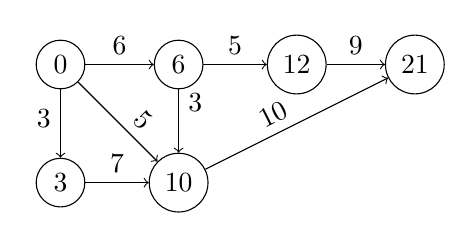
\begin{tikzpicture}[main/.style = {draw, circle},node distance={15mm}] 
        \node[main] (1) []{$0$}; 
        \node[main] (2) [right of=1] {$6$}; 
        \node[main] (3) [right of=2] {$12$}; 
        \node[main] (4) [below of=1] {$3$};
        \node[main] (5) [right of=4] {$10$};
        \node[main] (6) [right of=3] {$21$};
        \draw[->] (1) -- node[midway, above, sloped, pos=0.5] {$6$} (2);
        \draw[->] (2) -- node[midway, above, sloped, pos=0.5] {$5$} (3);
        \draw[->] (3) -- node[midway, above, sloped, pos=0.5] {$9$} (6);
        \draw[->] (1) -- node[midway, above left, pos=0.7] {$3$} (4);
        \draw[->] (1) -- node[midway, above right, sloped, pos=0.5] {$5$} (5);
        \draw[->] (4) -- node[midway, above, sloped, pos=0.5] {$7$} (5);
        \draw[->] (2) -- node[midway, above right, pos=0.5] {$3$} (5);
        \draw[->] (5) -- node[midway, above right, sloped, pos=0.3] {$10$} (6);
        \end{tikzpicture} 
    \end{center}

В задаче, которую мы будем рассматривать, граф уже топологически отсортирован. Это вызвано тем, что в данном графе будет выполнено условие: если $(x,y) \in E$, то $x < y$. 

\begin{verbatim}
#include <bits/stdc++.h>
using namespace std;
typedef long long ll;
const ll INF = 1'000'000'000'000'000'000; // очень большое число 
struct Edge{
    int y;
    ll w;
};
int n,m;
vector<vector<int>>color;
vector<vector<Edge>>e;

int main() {
    ios::sync_with_stdio(0);
    cin.tie(0);
    cout.tie(0);
    cin >> n >> m;
    e = vector<vector<Edge>>(n+1);
    for(int i = 1; i <= m; i++) {
        int x,y;
        ll w;
        cin >> x >> y >> w; // считываем ребра и вес
        e[x].push_back({y,w});
    }
    vector<ll>d(n+1, -INF); // изначально ставим -INF в вершину, это значит, что мы там не были
    d[1] = 0; // ставим первое значение, его мы знаем
    for(int x = 1; x <= n; i++) { // фиксируем вершину
        if(d[x] == -INF) continue; // если вершина не посещена, то не будем смотреть из нее пути
        for(auto& [y,w] : e[x]) { // идем во все вершины из нее
            d[y] = max(d[y], d[x] + w); 
        }
    }
    cout << d[n] << '\n';
}
\end{verbatim}

Простое решение, правда? Если вы хотите написать с рекурсией, то вот так это выглядит: 

\begin{verbatim}
#include <bits/stdc++.h>
using namespace std;
typedef long long ll;
const ll INF = 1'000'000'000'000'000'000; // очень большое число 
struct Edge{
    int y;
    ll w;
};
int n,m;
vector<vector<int>>color;
vector<vector<Edge>>e;
vector<int>color;
vector<ll>d;
void dfs(int x) {
    if(color[x]) return;
    color[x] = 1;
    for(auto& [y,w] : e[x]) {
        dfs(y);
        d[x] = max(d[x], d[y] + w);
    }
}
int main() {
    ios::sync_with_stdio(0);
    cin.tie(0);
    cout.tie(0);
    cin >> n >> m;
    e = vector<vector<Edge>>(n+1);
    for(int i = 1; i <= m; i++) {
        int x,y;
        ll w;
        cin >> x >> y >> w; // считываем ребра и вес
        e[x].push_back({y,w});
    }
    d = vector<ll>(n+1,-INF);
    color = vector<int>(n+1,0);
    color[n] = 1;
    d[n] = 0;
    for(int x = 1; x <= n; x++) {
        dfs(x);
    }
    cout << d[1] << '\n'; 
}
\end{verbatim}
В этом решении мы считали, что $d[x]$ равно максимальному пути из вершины $x$ в вершину $n$. Первый способ работает, потому что $[1,2,3,\ldots,n]$ является топсортом по условию задачи. Если же это не так, то можно найти топсорт и решение будет выглядеть так:

\begin{verbatim}
#include <bits/stdc++.h>
using namespace std;
typedef long long ll;
const ll INF = 1'000'000'000'000'000'000; // очень большое число 
struct Edge{
    int y;
    ll w;
};
int n,m;
vector<vector<int>>color;
vector<vector<Edge>>e;

vector<int>color;
void dfs(int x) {
    if(color[x]) return;
    color[x] = 1;
    for(auto& y : e[x]) {
        dfs(y);
    }
    path.push_back(x);
}
void topsort() {
    path = vector<int>();
    color = vector<int>(n+1);
    for(int i = 1; i <= n; i++) {
        dfs(i);
    }
    reverse(path.begin(),path.end());
}

int main() {
    ios::sync_with_stdio(0);
    cin.tie(0);
    cout.tie(0);
    cin >> n >> m;
    e = vector<vector<Edge>>(n+1);
    for(int i = 1; i <= m; i++) {
        int x,y;
        ll w;
        cin >> x >> y >> w; // считываем ребра и вес
        e[x].push_back({y,w});
    }
    vector<ll>d(n+1, -INF); // изначально ставим -INF в вершину, это значит, что мы там не были
    d[1] = 0; // ставим первое значение, его мы знаем
    topsort();
    for(auto& x : path) { // фиксируем вершину
        if(d[x] == -INF) continue; // если вершина не посещена, то не будем смотреть из нее пути
        for(auto& [y,w] : e[x]) { // идем во все вершины из нее
            d[y] = max(d[y], d[x] + w); 
        }
    }
    cout << d[n] << '\n';
}
\end{verbatim}

Решим следующую часто встречающуюся задачу: вам дан орграф со свойством: если $(x,y) \in E$, то $x < y$. Вам нужно найти путь из $1$ в $n$, который максимизирует минимум, то есть вам нужно найти $max(min(...))$. Смотрите: пусть ответ на задачу это число $A$ (это максимальный минимум на каком-то пути). Тогда попробуем решать задачу, отвечая на вопрос: есть ли такой путь, что мы получим ответ хотя бы $T$? Пусть $f(T)$ это ответ (да или нет). Тогда: $f(1), f(2), \ldots, f(A)$ это всегда истина, а $f(A+1),f(A+2),\ldots$ всегда ложь. Мы имеем функцию, по которой можно сделать бинпоиск. Тогда мы хотим, чтобы минимум на пути был хотя бы $T$, но если минимум на пути уже не меньше $T$, то все числа на этом пути не меньше $T$. Пишем решение:

\begin{verbatim}
#include <bits/stdc++.h>
using namespace std;
typedef long long ll;
const ll INF = 1'000'000'000'000'000'000; // очень большое число 
struct Edge{
    int y;
    ll w;
};
int n,m;
vector<vector<int>>color;
vector<vector<Edge>>e;

bool fun(int T) {
    color = vector<int>(n+1);
    color[1] = 1;
    for(int x = 1; x <= n; x++) {
        if(!color[x]) continue;
        for(auto& [y,w] : e[x]) {
            if(w < T) continue;
            color[y] = 1;
        }
    }
    return color[n];
}
int main() {
    ios::sync_with_stdio(0);
    cin.tie(0);
    cout.tie(0);
    cin >> n >> m;
    e = vector<vector<Edge>>(n+1);
    for(int i = 1; i <= m; i++) {
        int x,y;
        ll w;
        cin >> x >> y >> w; // считываем ребра и вес
        e[x].push_back({y,w});
    }
    int l = 1, r = 1'000'000'000 + 1;
    while(l + 1 < r){
        int h = (l+r)/2;
        if(fun(h)) l = h;
        else r = h;
    }
    cout << l << '\n';
}
\end{verbatim}

    
\end{document}
